\documentclass[a4paper]{book}
\usepackage{makeidx}
\usepackage{natbib}
\usepackage{graphicx}
\usepackage{multicol}
\usepackage{float}
\usepackage{listings}
\usepackage{color}
\usepackage{ifthen}
\usepackage[table]{xcolor}
\usepackage{textcomp}
\usepackage{alltt}
\usepackage{ifpdf}
\ifpdf
\usepackage[pdftex,
            pagebackref=true,
            colorlinks=true,
            linkcolor=blue,
            unicode
           ]{hyperref}
\else
\usepackage[ps2pdf,
            pagebackref=true,
            colorlinks=true,
            linkcolor=blue,
            unicode
           ]{hyperref}
\usepackage{pspicture}
\fi
\usepackage[utf8]{inputenc}
\usepackage{mathptmx}
\usepackage[scaled=.90]{helvet}
\usepackage{courier}
\usepackage{sectsty}
\usepackage[titles]{tocloft}
\usepackage{doxygen}
\lstset{language=C++,inputencoding=utf8,basicstyle=\footnotesize,breaklines=true,breakatwhitespace=true,tabsize=8,numbers=left }
\makeindex
\setcounter{tocdepth}{3}
\renewcommand{\footrulewidth}{0.4pt}
\renewcommand{\familydefault}{\sfdefault}
\hfuzz=15pt
\setlength{\emergencystretch}{15pt}
\hbadness=750
\tolerance=750
\begin{document}
\hypersetup{pageanchor=false,citecolor=blue}
\begin{titlepage}
\vspace*{7cm}
\begin{center}
{\Large \-S\-O\-Mtk }\\
\vspace*{1cm}
{\large \-Generated by Doxygen 1.7.6.1}\\
\vspace*{0.5cm}
{\small Thu Apr 12 2012 10:59:30}\\
\end{center}
\end{titlepage}
\clearemptydoublepage
\pagenumbering{roman}
\tableofcontents
\clearemptydoublepage
\pagenumbering{arabic}
\hypersetup{pageanchor=true,citecolor=blue}
\chapter{\-Todo \-List}
\label{todo}
\hypertarget{todo}{}

\begin{DoxyRefList}
\item[\label{todo__todo000003}%
\hypertarget{todo__todo000003}{}%
\-Member \hyperlink{classhsom_1_1_a_n_n_classifier_a2777506e21fc1fcb2900ede529aaefac}{hsom\-:\-:\-A\-N\-N\-Classifier\-:\-:classify} (\-Suspect\-Ptr suspect)]\-Move the input and output width parameters down into the base class 

ensure that the output widths match  
\item[\label{todo__todo000001}%
\hypertarget{todo__todo000001}{}%
\-Member \hyperlink{classhsom_1_1_a_n_n_classifier_a615dc19a6aa3f45ee00926e2707386e0}{hsom\-:\-:\-A\-N\-N\-Classifier\-:\-:read\-Classifier\-Data} (\-Q\-Dom\-Element \&element)]\-Insert some sort of verification here to make sure that the load went ok  
\item[\label{todo__todo000002}%
\hypertarget{todo__todo000002}{}%
\-Member \hyperlink{classhsom_1_1_a_n_n_classifier_ac3f43b1ab6681ad13acc52924e3c3fc5}{hsom\-:\-:\-A\-N\-N\-Classifier\-:\-:train\-Classifier} (\-Q\-Vector$<$ Suspect\-Ptr $>$ suspects, \-Q\-Map$<$ Q\-String, Q\-Variant $>$ training\-Parameters)]\-Move the input and output width parameters down into the base class  
\item[\label{todo__todo000006}%
\hypertarget{todo__todo000006}{}%
\-Member \hyperlink{classhsom_1_1_fast_hex_grid_a7fc65f0095eb0b5e14d41b116ea140d4}{hsom\-:\-:\-Fast\-Hex\-Grid$<$ \-T $>$\-:\-:diagonal} ()]\-Come up with a more precise computation of this 

\-Come up with a more precise computation of this  
\item[\label{todo__todo000005}%
\hypertarget{todo__todo000005}{}%
\-Member \hyperlink{classhsom_1_1_feature_afef971a3f4a596af3b7f6bfa8dd77341}{hsom\-:\-:\-Feature\-:\-:distance} (\-Feature other) const ]\-: make sure that the two features are the same size!  
\item[\label{todo__todo000007}%
\hypertarget{todo__todo000007}{}%
\-Member \hyperlink{classhsom_1_1_grid_ac4d7188e7b75823a03a53317656473fa}{hsom\-:\-:\-Grid$<$ \-T $>$\-:\-:operator\mbox{[}\mbox{]}} (int idx)]\-Add a bounds checking here and custom exceptions would be nice  
\item[\label{todo__todo000008}%
\hypertarget{todo__todo000008}{}%
\-Member \hyperlink{classhsom_1_1_hex_grid_aa1fe9291ee1c82da00bca12b906959cb}{hsom\-:\-:\-Hex\-Grid$<$ \-T $>$\-:\-:diagonal} ()]\-Come up with a more precise computation of this  
\item[\label{todo__todo000012}%
\hypertarget{todo__todo000012}{}%
\-Member \hyperlink{classhsom_1_1_histogram_a8f4a1e9947fa29a974e550c0b97f7496}{hsom\-:\-:\-Histogram\-:\-:normalize} ()]\-Add a parameter to choose normalization method 

investigate other normalizations.  
\item[\label{todo__todo000014}%
\hypertarget{todo__todo000014}{}%
\-Class \hyperlink{classhsom_1_1_h_s_o_m}{hsom\-:\-:\-H\-S\-O\-M} ]\-Implement this as a thread so that training can run in the background  
\item[\label{todo__todo000015}%
\hypertarget{todo__todo000015}{}%
\-Class \hyperlink{classhsom_1_1_normalizer}{hsom\-:\-:\-Normalizer} ]\-Document \-Classes and files  
\item[\label{todo__todo000009}%
\hypertarget{todo__todo000009}{}%
\-Member \hyperlink{classhsom_1_1_quad_grid_a8f5bc5583e2d254f3850dfa0542a5505}{hsom\-:\-:\-Quad\-Grid$<$ \-T $>$\-:\-:diagonal} ()]\-Come up with a more precise computation of this  
\item[\label{todo__todo000016}%
\hypertarget{todo__todo000016}{}%
\-Member \hyperlink{classhsom_1_1_s_o_m_ab49f133b064128ddce266f806ece2229}{hsom\-:\-:\-S\-O\-M\-:\-:initialize\-Training} (\-Q\-Map$<$ Q\-String, Q\-Variant $>$ som\-Parameters, \-Normalizer\-Ptr normalizer, int feature\-Size)]\-Add range check to alpha (hint on values) 

\-Perhaps use default values if the parameters aren't specified 

determine if there should be other constraints to alpha and radius ratio (negatives, ffs!) 
\end{DoxyRefList}
\chapter{\-Class \-Index}
\section{\-Class \-Hierarchy}
\-This inheritance list is sorted roughly, but not completely, alphabetically\-:\begin{DoxyCompactList}
\item \contentsline{section}{hsom\-:\-:\-Classifier}{\pageref{classhsom_1_1_classifier}}{}
\begin{DoxyCompactList}
\item \contentsline{section}{hsom\-:\-:\-A\-N\-N\-Classifier}{\pageref{classhsom_1_1_a_n_n_classifier}}{}
\end{DoxyCompactList}
\item \contentsline{section}{\-Color\-Suspect}{\pageref{class_color_suspect}}{}
\item \contentsline{section}{somtk\-:\-:\-Feature}{\pageref{classsomtk_1_1_feature}}{}
\item \contentsline{section}{somtk\-:\-:\-Grid$<$ \-T $>$}{\pageref{classsomtk_1_1_grid}}{}
\begin{DoxyCompactList}
\item \contentsline{section}{somtk\-:\-:\-Fast\-Hex\-Grid$<$ \-T $>$}{\pageref{classsomtk_1_1_fast_hex_grid}}{}
\begin{DoxyCompactList}
\item \contentsline{section}{somtk\-:\-:\-Wrap\-Hex\-Grid$<$ \-T $>$}{\pageref{classsomtk_1_1_wrap_hex_grid}}{}
\end{DoxyCompactList}
\item \contentsline{section}{somtk\-:\-:\-Hex\-Grid$<$ \-T $>$}{\pageref{classsomtk_1_1_hex_grid}}{}
\item \contentsline{section}{somtk\-:\-:\-Quad\-Grid$<$ \-T $>$}{\pageref{classsomtk_1_1_quad_grid}}{}
\end{DoxyCompactList}
\item \contentsline{section}{somtk\-:\-:\-Grid$<$ double $>$}{\pageref{classsomtk_1_1_grid}}{}
\begin{DoxyCompactList}
\item \contentsline{section}{somtk\-:\-:\-Hex\-Grid$<$ double $>$}{\pageref{classsomtk_1_1_hex_grid}}{}
\begin{DoxyCompactList}
\item \contentsline{section}{somtk\-:\-:\-Histogram}{\pageref{classsomtk_1_1_histogram}}{}
\end{DoxyCompactList}
\end{DoxyCompactList}
\item \contentsline{section}{somtk\-:\-:\-H\-S\-O\-M}{\pageref{classsomtk_1_1_h_s_o_m}}{}
\item \contentsline{section}{somtk\-:\-:\-Normalizer}{\pageref{classsomtk_1_1_normalizer}}{}
\begin{DoxyCompactList}
\item \contentsline{section}{somtk\-:\-:\-Min\-Max\-Normalizer}{\pageref{classsomtk_1_1_min_max_normalizer}}{}
\item \contentsline{section}{somtk\-:\-:\-Null\-Normalizer}{\pageref{classsomtk_1_1_null_normalizer}}{}
\item \contentsline{section}{somtk\-:\-:\-Sigmoid\-Normalizer}{\pageref{classsomtk_1_1_sigmoid_normalizer}}{}
\end{DoxyCompactList}
\item \contentsline{section}{somtk\-:\-:\-S\-O\-M}{\pageref{classsomtk_1_1_s_o_m}}{}
\item \contentsline{section}{somtk\-:\-:\-S\-O\-M\-Error}{\pageref{classsomtk_1_1_s_o_m_error}}{}
\end{DoxyCompactList}

\chapter{\-Class \-Index}
\section{\-Class \-List}
\-Here are the classes, structs, unions and interfaces with brief descriptions\-:\begin{DoxyCompactList}
\item\contentsline{section}{\hyperlink{classhsom_1_1_a_n_n_classifier}{hsom\-::\-A\-N\-N\-Classifier} }{\pageref{classhsom_1_1_a_n_n_classifier}}{}
\item\contentsline{section}{\hyperlink{classhsom_1_1_classifier}{hsom\-::\-Classifier} }{\pageref{classhsom_1_1_classifier}}{}
\item\contentsline{section}{\hyperlink{class_color_suspect}{\-Color\-Suspect} }{\pageref{class_color_suspect}}{}
\item\contentsline{section}{\hyperlink{classsomtk_1_1_fast_hex_grid}{somtk\-::\-Fast\-Hex\-Grid$<$ T $>$} }{\pageref{classsomtk_1_1_fast_hex_grid}}{}
\item\contentsline{section}{\hyperlink{classsomtk_1_1_feature}{somtk\-::\-Feature} \\*\-The feature class provides an abstract base class for \hyperlink{classsomtk_1_1_s_o_m}{\-S\-O\-M} features }{\pageref{classsomtk_1_1_feature}}{}
\item\contentsline{section}{\hyperlink{classsomtk_1_1_grid}{somtk\-::\-Grid$<$ T $>$} }{\pageref{classsomtk_1_1_grid}}{}
\item\contentsline{section}{\hyperlink{classsomtk_1_1_hex_grid}{somtk\-::\-Hex\-Grid$<$ T $>$} }{\pageref{classsomtk_1_1_hex_grid}}{}
\item\contentsline{section}{\hyperlink{classsomtk_1_1_histogram}{somtk\-::\-Histogram} }{\pageref{classsomtk_1_1_histogram}}{}
\item\contentsline{section}{\hyperlink{classsomtk_1_1_h_s_o_m}{somtk\-::\-H\-S\-O\-M} \\*\-The \hyperlink{classsomtk_1_1_s_o_m}{\-S\-O\-M} class provides an abstract base class for \-Self-\/\-Organizing \-Maps }{\pageref{classsomtk_1_1_h_s_o_m}}{}
\item\contentsline{section}{\hyperlink{classsomtk_1_1_min_max_normalizer}{somtk\-::\-Min\-Max\-Normalizer} }{\pageref{classsomtk_1_1_min_max_normalizer}}{}
\item\contentsline{section}{\hyperlink{classsomtk_1_1_normalizer}{somtk\-::\-Normalizer} }{\pageref{classsomtk_1_1_normalizer}}{}
\item\contentsline{section}{\hyperlink{classsomtk_1_1_null_normalizer}{somtk\-::\-Null\-Normalizer} }{\pageref{classsomtk_1_1_null_normalizer}}{}
\item\contentsline{section}{\hyperlink{classsomtk_1_1_quad_grid}{somtk\-::\-Quad\-Grid$<$ T $>$} }{\pageref{classsomtk_1_1_quad_grid}}{}
\item\contentsline{section}{\hyperlink{classsomtk_1_1_sigmoid_normalizer}{somtk\-::\-Sigmoid\-Normalizer} }{\pageref{classsomtk_1_1_sigmoid_normalizer}}{}
\item\contentsline{section}{\hyperlink{classsomtk_1_1_s_o_m}{somtk\-::\-S\-O\-M} }{\pageref{classsomtk_1_1_s_o_m}}{}
\item\contentsline{section}{\hyperlink{classsomtk_1_1_s_o_m_error}{somtk\-::\-S\-O\-M\-Error} }{\pageref{classsomtk_1_1_s_o_m_error}}{}
\item\contentsline{section}{\hyperlink{classsomtk_1_1_wrap_hex_grid}{somtk\-::\-Wrap\-Hex\-Grid$<$ T $>$} }{\pageref{classsomtk_1_1_wrap_hex_grid}}{}
\end{DoxyCompactList}

\chapter{\-Class \-Documentation}
\hypertarget{classhsom_1_1_a_n_n_classifier}{\section{hsom\-:\-:\-A\-N\-N\-Classifier \-Class \-Reference}
\label{classhsom_1_1_a_n_n_classifier}\index{hsom\-::\-A\-N\-N\-Classifier@{hsom\-::\-A\-N\-N\-Classifier}}
}
\-Inheritance diagram for hsom\-:\-:\-A\-N\-N\-Classifier\-:\begin{figure}[H]
\begin{center}
\leavevmode
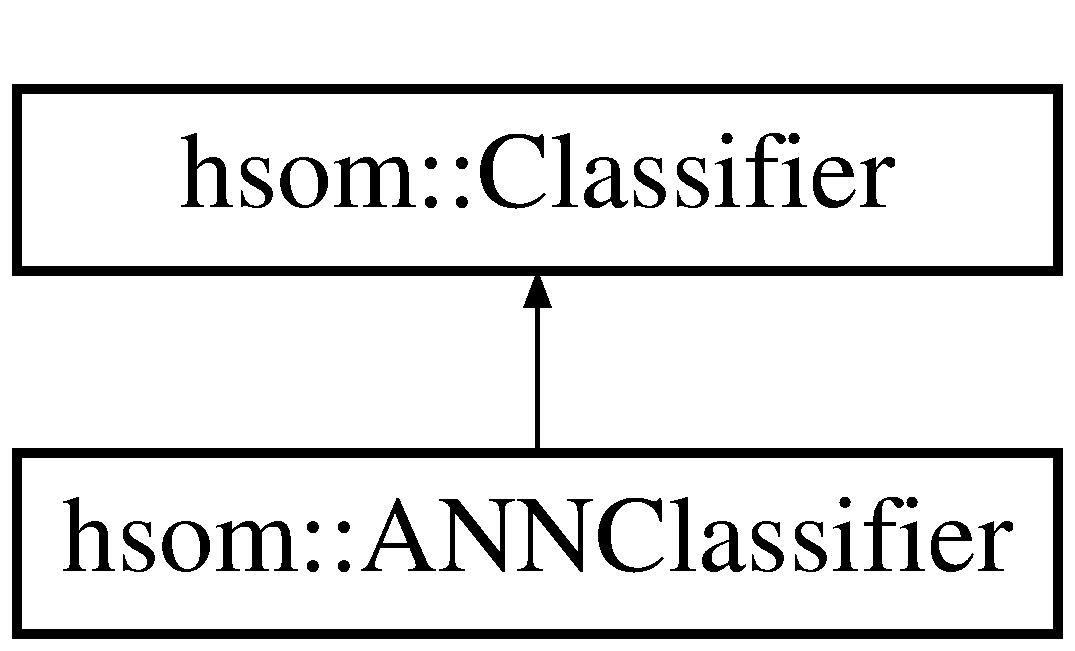
\includegraphics[height=2.000000cm]{classhsom_1_1_a_n_n_classifier}
\end{center}
\end{figure}
\subsection*{\-Public \-Member \-Functions}
\begin{DoxyCompactItemize}
\item 
\hypertarget{classhsom_1_1_a_n_n_classifier_a1af6ffad791c85dd9629131c5c5020f9}{{\bfseries \-A\-N\-N\-Classifier} (\-Q\-String file\-Name)}\label{classhsom_1_1_a_n_n_classifier_a1af6ffad791c85dd9629131c5c5020f9}

\item 
virtual void \hyperlink{classhsom_1_1_a_n_n_classifier_a2777506e21fc1fcb2900ede529aaefac}{classify} (\-Suspect\-Ptr suspect)
\begin{DoxyCompactList}\small\item\em \-Classifies a single suspect. \end{DoxyCompactList}\end{DoxyCompactItemize}
\subsection*{\-Protected \-Member \-Functions}
\begin{DoxyCompactItemize}
\item 
virtual void \hyperlink{classhsom_1_1_a_n_n_classifier_a615dc19a6aa3f45ee00926e2707386e0}{read\-Classifier\-Data} (\-Q\-Dom\-Element \&element)
\begin{DoxyCompactList}\small\item\em \-Interfaces with the \-Persist\-X\-M\-L \-A\-P\-I to ensure correct loading order for a classifier. \end{DoxyCompactList}\item 
virtual void \hyperlink{classhsom_1_1_a_n_n_classifier_a16189d3191b92fefe2f3103b5b789a9d}{write\-Classifier\-Data} (\-Q\-Dom\-Element \&element)
\begin{DoxyCompactList}\small\item\em \-Interfaces with the \-Persist\-X\-M\-L \-A\-P\-I to ensure correct saving order for a classifier. \end{DoxyCompactList}\item 
virtual void \hyperlink{classhsom_1_1_a_n_n_classifier_ac3f43b1ab6681ad13acc52924e3c3fc5}{train\-Classifier} (\-Q\-Vector$<$ \-Suspect\-Ptr $>$ suspects, \-Q\-Map$<$ \-Q\-String, \-Q\-Variant $>$ training\-Parameters)
\begin{DoxyCompactList}\small\item\em \-Performs specific training algorithm for a classifier. \end{DoxyCompactList}\end{DoxyCompactItemize}


\subsection{\-Member \-Function \-Documentation}
\hypertarget{classhsom_1_1_a_n_n_classifier_a2777506e21fc1fcb2900ede529aaefac}{\index{hsom\-::\-A\-N\-N\-Classifier@{hsom\-::\-A\-N\-N\-Classifier}!classify@{classify}}
\index{classify@{classify}!hsom::ANNClassifier@{hsom\-::\-A\-N\-N\-Classifier}}
\subsubsection[{classify}]{\setlength{\rightskip}{0pt plus 5cm}void {\bf hsom\-::\-A\-N\-N\-Classifier\-::classify} (
\begin{DoxyParamCaption}
\item[{\-Suspect\-Ptr}]{suspect}
\end{DoxyParamCaption}
)\hspace{0.3cm}{\ttfamily  \mbox{[}virtual\mbox{]}}}}\label{classhsom_1_1_a_n_n_classifier_a2777506e21fc1fcb2900ede529aaefac}


\-Classifies a single suspect. 

\begin{DoxyRefDesc}{\-Todo}
\item[\hyperlink{todo__todo000003}{\-Todo}]\-Move the input and output width parameters down into the base class \end{DoxyRefDesc}


\begin{DoxyRefDesc}{\-Todo}
\item[\hyperlink{todo__todo000004}{\-Todo}]ensure that the output widths match \end{DoxyRefDesc}


\-Implements \hyperlink{classhsom_1_1_classifier_afe72e6af42ffe1bc2921b3ade481d800}{hsom\-::\-Classifier}.

\hypertarget{classhsom_1_1_a_n_n_classifier_a615dc19a6aa3f45ee00926e2707386e0}{\index{hsom\-::\-A\-N\-N\-Classifier@{hsom\-::\-A\-N\-N\-Classifier}!read\-Classifier\-Data@{read\-Classifier\-Data}}
\index{read\-Classifier\-Data@{read\-Classifier\-Data}!hsom::ANNClassifier@{hsom\-::\-A\-N\-N\-Classifier}}
\subsubsection[{read\-Classifier\-Data}]{\setlength{\rightskip}{0pt plus 5cm}void {\bf hsom\-::\-A\-N\-N\-Classifier\-::read\-Classifier\-Data} (
\begin{DoxyParamCaption}
\item[{\-Q\-Dom\-Element \&}]{element}
\end{DoxyParamCaption}
)\hspace{0.3cm}{\ttfamily  \mbox{[}protected, virtual\mbox{]}}}}\label{classhsom_1_1_a_n_n_classifier_a615dc19a6aa3f45ee00926e2707386e0}


\-Interfaces with the \-Persist\-X\-M\-L \-A\-P\-I to ensure correct loading order for a classifier. 

\begin{DoxyNote}{\-Note}
\-This is optional. \-If not implemented by a derived class, this function does nothing 
\end{DoxyNote}
\begin{DoxyRefDesc}{\-Todo}
\item[\hyperlink{todo__todo000001}{\-Todo}]\-Insert some sort of verification here to make sure that the load went ok \end{DoxyRefDesc}


\-Reimplemented from \hyperlink{classhsom_1_1_classifier_a7005afab0da6cfd49119ba21e31f0d35}{hsom\-::\-Classifier}.

\hypertarget{classhsom_1_1_a_n_n_classifier_ac3f43b1ab6681ad13acc52924e3c3fc5}{\index{hsom\-::\-A\-N\-N\-Classifier@{hsom\-::\-A\-N\-N\-Classifier}!train\-Classifier@{train\-Classifier}}
\index{train\-Classifier@{train\-Classifier}!hsom::ANNClassifier@{hsom\-::\-A\-N\-N\-Classifier}}
\subsubsection[{train\-Classifier}]{\setlength{\rightskip}{0pt plus 5cm}void {\bf hsom\-::\-A\-N\-N\-Classifier\-::train\-Classifier} (
\begin{DoxyParamCaption}
\item[{\-Q\-Vector$<$ \-Suspect\-Ptr $>$}]{suspects, }
\item[{\-Q\-Map$<$ \-Q\-String, \-Q\-Variant $>$}]{training\-Parameters}
\end{DoxyParamCaption}
)\hspace{0.3cm}{\ttfamily  \mbox{[}protected, virtual\mbox{]}}}}\label{classhsom_1_1_a_n_n_classifier_ac3f43b1ab6681ad13acc52924e3c3fc5}


\-Performs specific training algorithm for a classifier. 

\begin{DoxyRefDesc}{\-Todo}
\item[\hyperlink{todo__todo000002}{\-Todo}]\-Move the input and output width parameters down into the base class \end{DoxyRefDesc}


\-Implements \hyperlink{classhsom_1_1_classifier_a1f622d490d89f851c8641b0401648acb}{hsom\-::\-Classifier}.

\hypertarget{classhsom_1_1_a_n_n_classifier_a16189d3191b92fefe2f3103b5b789a9d}{\index{hsom\-::\-A\-N\-N\-Classifier@{hsom\-::\-A\-N\-N\-Classifier}!write\-Classifier\-Data@{write\-Classifier\-Data}}
\index{write\-Classifier\-Data@{write\-Classifier\-Data}!hsom::ANNClassifier@{hsom\-::\-A\-N\-N\-Classifier}}
\subsubsection[{write\-Classifier\-Data}]{\setlength{\rightskip}{0pt plus 5cm}void {\bf hsom\-::\-A\-N\-N\-Classifier\-::write\-Classifier\-Data} (
\begin{DoxyParamCaption}
\item[{\-Q\-Dom\-Element \&}]{element}
\end{DoxyParamCaption}
)\hspace{0.3cm}{\ttfamily  \mbox{[}protected, virtual\mbox{]}}}}\label{classhsom_1_1_a_n_n_classifier_a16189d3191b92fefe2f3103b5b789a9d}


\-Interfaces with the \-Persist\-X\-M\-L \-A\-P\-I to ensure correct saving order for a classifier. 

\begin{DoxyNote}{\-Note}
\-This is optional. \-If not implemented by a derived class, this function does nothing 
\end{DoxyNote}


\-Reimplemented from \hyperlink{classhsom_1_1_classifier_a44fd60ca14d06f5f3889e3d49573cd75}{hsom\-::\-Classifier}.



\-The documentation for this class was generated from the following files\-:\begin{DoxyCompactItemize}
\item 
\-C\-:/\-Users/d3x874/\-Documents/source/urania/classifiers/annclassifier.\-h\item 
\-C\-:/\-Users/d3x874/\-Documents/source/urania/classifiers/annclassifier.\-cpp\end{DoxyCompactItemize}

\hypertarget{classhsom_1_1_classifier}{\section{hsom\-:\-:\-Classifier \-Class \-Reference}
\label{classhsom_1_1_classifier}\index{hsom\-::\-Classifier@{hsom\-::\-Classifier}}
}
\-Inheritance diagram for hsom\-:\-:\-Classifier\-:\begin{figure}[H]
\begin{center}
\leavevmode
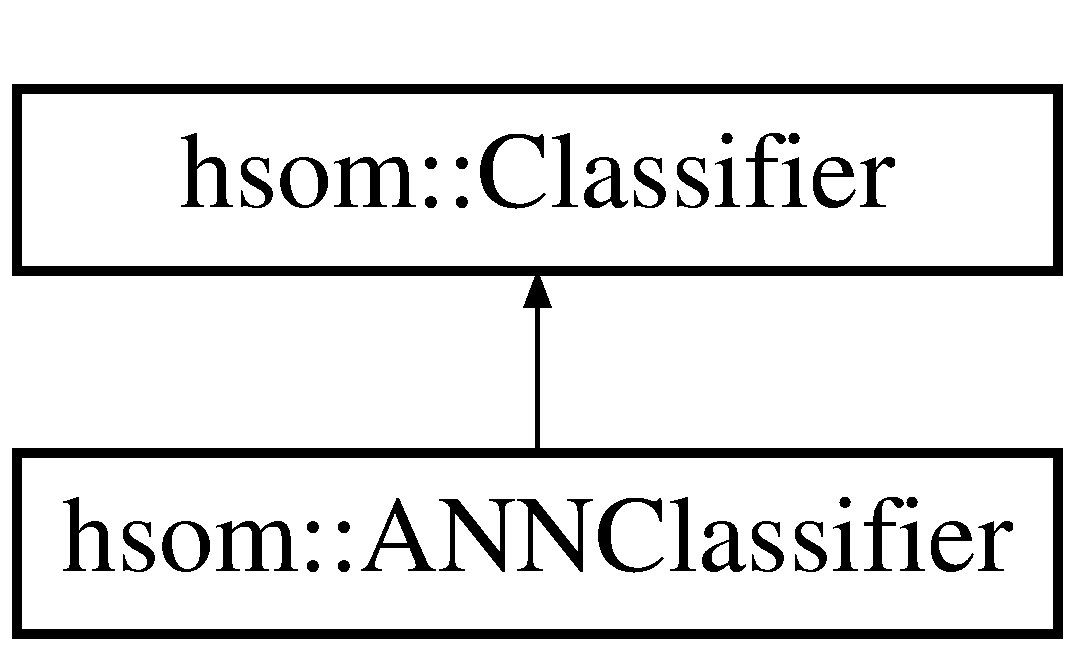
\includegraphics[height=2.000000cm]{classhsom_1_1_classifier}
\end{center}
\end{figure}
\subsection*{\-Public \-Member \-Functions}
\begin{DoxyCompactItemize}
\item 
\hypertarget{classhsom_1_1_classifier_a10514744eb67348a8dd8f71ec2c1631e}{\hyperlink{classhsom_1_1_classifier_a10514744eb67348a8dd8f71ec2c1631e}{\-Classifier} ()}\label{classhsom_1_1_classifier_a10514744eb67348a8dd8f71ec2c1631e}

\begin{DoxyCompactList}\small\item\em \-Constructs a classifier base instance. \end{DoxyCompactList}\item 
void \hyperlink{classhsom_1_1_classifier_a86175b0c10c80d7e0ea84e608ec49d19}{train} (\-Q\-Vector$<$ \-Suspect\-Ptr $>$ suspects, \-Q\-Map$<$ \-Q\-String, \-Q\-Variant $>$ training\-Parameters)
\begin{DoxyCompactList}\small\item\em \-Trains the classifier using a collection of known suspects. \end{DoxyCompactList}\item 
virtual void \hyperlink{classhsom_1_1_classifier_afe72e6af42ffe1bc2921b3ade481d800}{classify} (\-Suspect\-Ptr suspect)=0
\begin{DoxyCompactList}\small\item\em \-Classifies a single suspect. \end{DoxyCompactList}\item 
\hypertarget{classhsom_1_1_classifier_ad7a6005aea99220ef0391b1155310337}{virtual void {\bfseries read\-Data} (\-Q\-Dom\-Element \&element)}\label{classhsom_1_1_classifier_ad7a6005aea99220ef0391b1155310337}

\item 
\hypertarget{classhsom_1_1_classifier_a526942872ee1edea3ac51e37f0f45231}{virtual void {\bfseries write\-Data} (\-Q\-Dom\-Element \&element)}\label{classhsom_1_1_classifier_a526942872ee1edea3ac51e37f0f45231}

\end{DoxyCompactItemize}
\subsection*{\-Protected \-Member \-Functions}
\begin{DoxyCompactItemize}
\item 
virtual void \hyperlink{classhsom_1_1_classifier_a7005afab0da6cfd49119ba21e31f0d35}{read\-Classifier\-Data} (\-Q\-Dom\-Element \&element)
\begin{DoxyCompactList}\small\item\em \-Interfaces with the \-Persist\-X\-M\-L \-A\-P\-I to ensure correct loading order for a classifier. \end{DoxyCompactList}\item 
virtual void \hyperlink{classhsom_1_1_classifier_a44fd60ca14d06f5f3889e3d49573cd75}{write\-Classifier\-Data} (\-Q\-Dom\-Element \&element)
\begin{DoxyCompactList}\small\item\em \-Interfaces with the \-Persist\-X\-M\-L \-A\-P\-I to ensure correct saving order for a classifier. \end{DoxyCompactList}\item 
virtual void \hyperlink{classhsom_1_1_classifier_a1f622d490d89f851c8641b0401648acb}{train\-Classifier} (\-Q\-Vector$<$ \-Suspect\-Ptr $>$ suspects, \-Q\-Map$<$ \-Q\-String, \-Q\-Variant $>$ training\-Parameters)=0
\begin{DoxyCompactList}\small\item\em \-Performs specific training algorithm for a classifier. \end{DoxyCompactList}\end{DoxyCompactItemize}
\subsection*{\-Protected \-Attributes}
\begin{DoxyCompactItemize}
\item 
\hypertarget{classhsom_1_1_classifier_a57f42894e3369a20b4fd0f3dd8f3d8a5}{\-Q\-Map$<$ \-Q\-String, \-Q\-Variant $>$ \hyperlink{classhsom_1_1_classifier_a57f42894e3369a20b4fd0f3dd8f3d8a5}{\-\_\-training\-Parameters}}\label{classhsom_1_1_classifier_a57f42894e3369a20b4fd0f3dd8f3d8a5}

\begin{DoxyCompactList}\small\item\em \-Describes the parameters used to tune the training of this classifier. \end{DoxyCompactList}\end{DoxyCompactItemize}


\subsection{\-Member \-Function \-Documentation}
\hypertarget{classhsom_1_1_classifier_afe72e6af42ffe1bc2921b3ade481d800}{\index{hsom\-::\-Classifier@{hsom\-::\-Classifier}!classify@{classify}}
\index{classify@{classify}!hsom::Classifier@{hsom\-::\-Classifier}}
\subsubsection[{classify}]{\setlength{\rightskip}{0pt plus 5cm}virtual void {\bf hsom\-::\-Classifier\-::classify} (
\begin{DoxyParamCaption}
\item[{\-Suspect\-Ptr}]{suspect}
\end{DoxyParamCaption}
)\hspace{0.3cm}{\ttfamily  \mbox{[}pure virtual\mbox{]}}}}\label{classhsom_1_1_classifier_afe72e6af42ffe1bc2921b3ade481d800}


\-Classifies a single suspect. 


\begin{DoxyParams}{\-Parameters}
{\em suspect} & \-The suspect to be classified \\
\hline
\end{DoxyParams}


\-Implemented in \hyperlink{classhsom_1_1_a_n_n_classifier_a2777506e21fc1fcb2900ede529aaefac}{hsom\-::\-A\-N\-N\-Classifier}.

\hypertarget{classhsom_1_1_classifier_a7005afab0da6cfd49119ba21e31f0d35}{\index{hsom\-::\-Classifier@{hsom\-::\-Classifier}!read\-Classifier\-Data@{read\-Classifier\-Data}}
\index{read\-Classifier\-Data@{read\-Classifier\-Data}!hsom::Classifier@{hsom\-::\-Classifier}}
\subsubsection[{read\-Classifier\-Data}]{\setlength{\rightskip}{0pt plus 5cm}void {\bf hsom\-::\-Classifier\-::read\-Classifier\-Data} (
\begin{DoxyParamCaption}
\item[{\-Q\-Dom\-Element \&}]{element}
\end{DoxyParamCaption}
)\hspace{0.3cm}{\ttfamily  \mbox{[}protected, virtual\mbox{]}}}}\label{classhsom_1_1_classifier_a7005afab0da6cfd49119ba21e31f0d35}


\-Interfaces with the \-Persist\-X\-M\-L \-A\-P\-I to ensure correct loading order for a classifier. 

\begin{DoxyNote}{\-Note}
\-This is optional. \-If not implemented by a derived class, this function does nothing 
\end{DoxyNote}


\-Reimplemented in \hyperlink{classhsom_1_1_a_n_n_classifier_a615dc19a6aa3f45ee00926e2707386e0}{hsom\-::\-A\-N\-N\-Classifier}.

\hypertarget{classhsom_1_1_classifier_a86175b0c10c80d7e0ea84e608ec49d19}{\index{hsom\-::\-Classifier@{hsom\-::\-Classifier}!train@{train}}
\index{train@{train}!hsom::Classifier@{hsom\-::\-Classifier}}
\subsubsection[{train}]{\setlength{\rightskip}{0pt plus 5cm}void {\bf hsom\-::\-Classifier\-::train} (
\begin{DoxyParamCaption}
\item[{\-Q\-Vector$<$ \-Suspect\-Ptr $>$}]{suspects, }
\item[{\-Q\-Map$<$ \-Q\-String, \-Q\-Variant $>$}]{training\-Parameters}
\end{DoxyParamCaption}
)}}\label{classhsom_1_1_classifier_a86175b0c10c80d7e0ea84e608ec49d19}


\-Trains the classifier using a collection of known suspects. 


\begin{DoxyParams}{\-Parameters}
{\em suspects} & \-The list of suspects with which to train this classifier \\
\hline
{\em training\-Parameters} & \-The tuning parameters used to train this classifier \\
\hline
\end{DoxyParams}
\hypertarget{classhsom_1_1_classifier_a1f622d490d89f851c8641b0401648acb}{\index{hsom\-::\-Classifier@{hsom\-::\-Classifier}!train\-Classifier@{train\-Classifier}}
\index{train\-Classifier@{train\-Classifier}!hsom::Classifier@{hsom\-::\-Classifier}}
\subsubsection[{train\-Classifier}]{\setlength{\rightskip}{0pt plus 5cm}virtual void {\bf hsom\-::\-Classifier\-::train\-Classifier} (
\begin{DoxyParamCaption}
\item[{\-Q\-Vector$<$ \-Suspect\-Ptr $>$}]{suspects, }
\item[{\-Q\-Map$<$ \-Q\-String, \-Q\-Variant $>$}]{training\-Parameters}
\end{DoxyParamCaption}
)\hspace{0.3cm}{\ttfamily  \mbox{[}protected, pure virtual\mbox{]}}}}\label{classhsom_1_1_classifier_a1f622d490d89f851c8641b0401648acb}


\-Performs specific training algorithm for a classifier. 


\begin{DoxyParams}{\-Parameters}
{\em suspects} & \-The list of suspects with which to train this classifier \\
\hline
{\em training\-Parameters} & \-The tuning parameters used to train this classifier \\
\hline
\end{DoxyParams}


\-Implemented in \hyperlink{classhsom_1_1_a_n_n_classifier_ac3f43b1ab6681ad13acc52924e3c3fc5}{hsom\-::\-A\-N\-N\-Classifier}.

\hypertarget{classhsom_1_1_classifier_a44fd60ca14d06f5f3889e3d49573cd75}{\index{hsom\-::\-Classifier@{hsom\-::\-Classifier}!write\-Classifier\-Data@{write\-Classifier\-Data}}
\index{write\-Classifier\-Data@{write\-Classifier\-Data}!hsom::Classifier@{hsom\-::\-Classifier}}
\subsubsection[{write\-Classifier\-Data}]{\setlength{\rightskip}{0pt plus 5cm}void {\bf hsom\-::\-Classifier\-::write\-Classifier\-Data} (
\begin{DoxyParamCaption}
\item[{\-Q\-Dom\-Element \&}]{element}
\end{DoxyParamCaption}
)\hspace{0.3cm}{\ttfamily  \mbox{[}protected, virtual\mbox{]}}}}\label{classhsom_1_1_classifier_a44fd60ca14d06f5f3889e3d49573cd75}


\-Interfaces with the \-Persist\-X\-M\-L \-A\-P\-I to ensure correct saving order for a classifier. 

\begin{DoxyNote}{\-Note}
\-This is optional. \-If not implemented by a derived class, this function does nothing 
\end{DoxyNote}


\-Reimplemented in \hyperlink{classhsom_1_1_a_n_n_classifier_a16189d3191b92fefe2f3103b5b789a9d}{hsom\-::\-A\-N\-N\-Classifier}.



\-The documentation for this class was generated from the following files\-:\begin{DoxyCompactItemize}
\item 
\-C\-:/\-Users/d3x874/\-Documents/source/urania/classifiers/classifier.\-h\item 
\-C\-:/\-Users/d3x874/\-Documents/source/urania/classifiers/classifier.\-cpp\end{DoxyCompactItemize}

\hypertarget{class_color_suspect}{\section{\-Color\-Suspect \-Class \-Reference}
\label{class_color_suspect}\index{\-Color\-Suspect@{\-Color\-Suspect}}
}
\subsection*{\-Public \-Member \-Functions}
\begin{DoxyCompactItemize}
\item 
\hyperlink{class_color_suspect_afbbbbd9c577ff42ecada23b497a451cb}{\-Color\-Suspect} (const cv\-::\-Mat \&img, int real\-Cat, int cat\-Ct, const \-Size\-Plus$<$ int $>$ \&hist\-Sz, std\-::string name)
\item 
virtual \hyperlink{class_color_suspect_acd02132c6855e7a8f63ddd8b5d790996}{$\sim$\-Color\-Suspect} ()
\item 
virtual \-Feature $\ast$ \hyperlink{class_color_suspect_ae9d514be897435ac42d73a7aed5bf855}{get\-Next\-Feature} ()
\end{DoxyCompactItemize}


\subsection{\-Constructor \& \-Destructor \-Documentation}
\hypertarget{class_color_suspect_afbbbbd9c577ff42ecada23b497a451cb}{\index{\-Color\-Suspect@{\-Color\-Suspect}!\-Color\-Suspect@{\-Color\-Suspect}}
\index{\-Color\-Suspect@{\-Color\-Suspect}!ColorSuspect@{\-Color\-Suspect}}
\subsubsection[{\-Color\-Suspect}]{\setlength{\rightskip}{0pt plus 5cm}\-Color\-Suspect\-::\-Color\-Suspect (
\begin{DoxyParamCaption}
\item[{const cv\-::\-Mat \&}]{img, }
\item[{int}]{real\-Cat, }
\item[{int}]{cat\-Ct, }
\item[{const \-Size\-Plus$<$ int $>$ \&}]{hist\-Sz, }
\item[{std\-::string}]{name}
\end{DoxyParamCaption}
)}}\label{class_color_suspect_afbbbbd9c577ff42ecada23b497a451cb}
\-Creates a new \hyperlink{class_color_suspect}{\-Color\-Suspect} 
\begin{DoxyParams}{\-Parameters}
{\em img} & -\/ \-The image that this \-Suspect represents \\
\hline
{\em real\-Cat} & -\/ \-The actual category for this \-Suspect \\
\hline
{\em cat\-Ct} & -\/ \-The number of categories possilbel for this \-Suspect \\
\hline
{\em grid\-Sz} & -\/ \-The size of this \-Suspect's histogram \\
\hline
{\em name} & -\/ \-The name of this \-Suspect \\
\hline
\end{DoxyParams}
\hypertarget{class_color_suspect_acd02132c6855e7a8f63ddd8b5d790996}{\index{\-Color\-Suspect@{\-Color\-Suspect}!$\sim$\-Color\-Suspect@{$\sim$\-Color\-Suspect}}
\index{$\sim$\-Color\-Suspect@{$\sim$\-Color\-Suspect}!ColorSuspect@{\-Color\-Suspect}}
\subsubsection[{$\sim$\-Color\-Suspect}]{\setlength{\rightskip}{0pt plus 5cm}{\bf \-Color\-Suspect\-::$\sim$\-Color\-Suspect} (
\begin{DoxyParamCaption}
{}
\end{DoxyParamCaption}
)\hspace{0.3cm}{\ttfamily  \mbox{[}virtual\mbox{]}}}}\label{class_color_suspect_acd02132c6855e7a8f63ddd8b5d790996}
\-Destructs this suspect 

\subsection{\-Member \-Function \-Documentation}
\hypertarget{class_color_suspect_ae9d514be897435ac42d73a7aed5bf855}{\index{\-Color\-Suspect@{\-Color\-Suspect}!get\-Next\-Feature@{get\-Next\-Feature}}
\index{get\-Next\-Feature@{get\-Next\-Feature}!ColorSuspect@{\-Color\-Suspect}}
\subsubsection[{get\-Next\-Feature}]{\setlength{\rightskip}{0pt plus 5cm}\-Feature $\ast$ {\bf \-Color\-Suspect\-::get\-Next\-Feature} (
\begin{DoxyParamCaption}
{}
\end{DoxyParamCaption}
)\hspace{0.3cm}{\ttfamily  \mbox{[}virtual\mbox{]}}}}\label{class_color_suspect_ae9d514be897435ac42d73a7aed5bf855}
\-Generates the next feature from this \-Suspect 

\-The documentation for this class was generated from the following files\-:\begin{DoxyCompactItemize}
\item 
\-C\-:/\-Users/d3x874/\-Documents/source/urania/suspects/colorsuspect.\-h\item 
\-C\-:/\-Users/d3x874/\-Documents/source/urania/suspects/colorsuspect.\-cpp\end{DoxyCompactItemize}

\input{classsomtk_1_1_fast_hex_grid}
\input{classsomtk_1_1_feature}
\input{classsomtk_1_1_grid}
\input{classsomtk_1_1_hex_grid}
\input{classsomtk_1_1_histogram}
\input{classsomtk_1_1_h_s_o_m}
\input{classsomtk_1_1_min_max_normalizer}
\input{classsomtk_1_1_normalizer}
\input{classsomtk_1_1_null_normalizer}
\input{classsomtk_1_1_quad_grid}
\input{classsomtk_1_1_sigmoid_normalizer}
\input{classsomtk_1_1_s_o_m}
\input{classsomtk_1_1_s_o_m_error}
\input{classsomtk_1_1_wrap_hex_grid}
\printindex
\end{document}
